\begin{table*}[!t]
    \caption{Active NLOS imaging \label{tab:active}}
    {\begin{tabular}{>{\raggedright}m{3.3cm}m{3.7cm}m{3cm}m{2cm}m{3cm}}%%%The number of columns has to be defined here
    \hline
    Reference & Illumination & Sensor & Information & Task\\ %%%% Table body
    \hline
    \cite{guptaReconstructionHidden3D2012,veltenRecoveringThreedimensionalShape2012} & Pulsed laser & Streak camera & Time of fight &  3D reconstruction\\%%%% Table body
    \cite{buttafavaNonlineofsightImagingUsing2015,laurenzisMultiplereturnSinglephotonCounting2015,heideNonlineofsightImagingPartial2017,jinReconstructionMultipleNonlineofsight2018,arellanoFastBackprojectionNonline2017,mannaErrorBackprojectionAlgorithms2018,otooleConfocalNonlineofsightImaging2018,Lindell:2019:Wave,tsaiVolumetricAlbedoSurface2019,pediredlaSNLOSNonlineofsightScanning2019,xinTheoryFermatPaths2019,musarraNonlineofsight3DImaging2019,liuVirtualWaveOptics2018,liuPhasorFieldDiffraction2020,Ahn_2019_ICCV,chopiteDeepNonLineofSightReconstruction2020,Young:2020:dlct,iseringhausen:2018,mannaNonlineofsightimagingUsingDynamic2020,liMambaTemporalConsistency2024,chen_learned_2020,yuLearnableInverseKernel2023,wuNonLineofsightImaging2021,yeCompressedSensingActive2021,isogawaTransientSinograms2020,wuMiniaturizedTCSPC2024,liuGeometricConstrainedNLOS2025,grauOcclusionFields2022,choiSelfCalibratingNLOS2023,guFastNLOSNonPlanar2023,sultanOptimizedSamplingNLOS2025,liDeepNLOSUnderscanning2023,yinAllDayNLOS2026,gaoLearnedLCT2026,sunTransVID2026,weiMultiSurfaceNLOS2025,luesiaStereoNLOS2026,zengCompactLongRangeNLOS2026,yangModelDecompositionNLOS2026,oyamaAdaptiveSpiralNLOS2026,liangFMCWNLOS2026,wangLaserReflectiveTomography2026,yuNonconfocalPhaseCompensation2026,tianSparseBayesianNLOS2026,zhouPolarizationSpeckleNLOS2026,miaoLaserPulseMultiplexingNLOS2026,weiQuasiFresnelNLOS2025,zhangFrequencyMoENLOS2026,chenCannyArtifactNLOS2026,shiSpecularFlightPathNLOS2026} & Pulsed laser & SPAD & Time of fight &  3D reconstruction\\%%%% Table body
    \cite{thrampoulidisExploitingOcclusionNonLineofSight2018,xuPhotonEfficientOcclusion2018} & Pulsed laser & SPAD & Integrated photon counts and occlusion & 2D reflectivity reconstruction\\%%%% Table body
    \cite{chanNonlineofsightTrackingPeople2017a,celebiHumanDetectionNLOS2026}(long range),\cite{caramazzaNeuralNetworkIdentification2017,musarraDetectionIdentificationTracking2019}(single point) & Pulsed laser & SPAD & Time of fight &  Detection/ Tracking/ Identification\\%%%% Table body
    \cite{isogawaOpticalNonLineofSightPhysicsBased2020,romanelliFiniteApertureYawNLOS2026,xiaoNLOSHumanPose2026} & Pulsed laser & SPAD & Time of fight &  Pose estimation\\%%%% Table body
    \cite{nam_real-time_2020,jinScannerlessNonlineofsightThree2020} & Pulsed laser & SPAD array & Time of fight &  3D reconstruction\\%%%% Table body
    \cite{gariepyDetectionTrackingMoving2016} & Pulsed laser & SPAD array & Time of fight &  Detection/ Tracking/ Identification\\%%%% Table body
    \cite{Willomitzer:18,xinTheoryFermatPaths2019,rezaPhasorFieldWaves2019} & Pulsed laser & Interferometer & Coherence &  3D reconstruction\\%%%% Table body
    \cite{heideDiffuseMirrors3D2014,kadambiOccludedImagingTimeofflight2016,caligiuriNIGHT2024} & Modulated laser & ToF camera & Time of fight &  3D reconstruction\\%%%% Table body
    \cite{zhuFastNonlineofsightImaging2021a} & Integrated & LiDAR & Depth and intensity &  3D reconstruction\\%%%% Table body
    \cite{chenSteadystateNonLineofSightImaging2019,vedaldi_imaging_2020} & Continuous laser & Conventional camera & Intensity &  3D reconstruction\\%%%% Table body
    \cite{kleinTrackingObjectsOutside2016,smithTrackingMultipleObjects2018a,leiDirectObjectRecognition2019} & Continuous laser & Conventional camera & Intensity &  Detection/ Tracking/ Identification\\%%%% Table body
    \cite{chandranAdaptiveLightingDataDriven2019} & Incoherent light source (imaging side) & Conventional camera & Intensity &  Detection/ Tracking/ Identification\\%%%% Table body
    \cite{DBLP:journals/corr/abs-1810-11710} & Incoherent light source (imaging side) & Conventional camera & Intensity &  2D reconstruction\\%%%% Table body
    \cite{Lindell:2019:Acoustic} & Speaker & Microphone & Acoustic "ToF" &  3D reconstruction\\%%%% Table body
    \hline
    \end{tabular}}{}
    \end{table*}%%%End of the table

\bookmark[dest=\HyperLocalCurrentHref,level=1]{Active Methods}
\section{Active Methods} \label{sec2}
Active NLOS imaging employs a controllable light source (usually a narrow-band laser) and a detector to obtain reflected information, which is then used to reconstruct hidden scenes. This section introduces recent advances of active NLOS imaging from three parts: hardware devices, physical light transport models, and reconstruction algorithms. Besides, the challenges and prospects of active NLOS imaging are analyzed at the end of the section. Table~\ref{tab:active} summarizes active imaging systems, where each row of the table lists the light source, sensor, information, and task for different NLOS imaging techniques.

\bookmark[dest=\HyperLocalCurrentHref,level=2]{Hardware Devices in Active Methods}
\subsection{Hardware Devices in Active Methods}
A variety of detectors, from professional interferometers~\cite{xinTheoryFermatPaths2019} and single-photon counters~\cite{buttafavaNonlineofsightImagingUsing2015,wang2021non} to ordinary cameras and even cell-phone cameras, have been used in NLOS imaging. Different detectors need to be combined with corresponding illumination sources to complete specific NLOS tasks. Here, we introduce such combinations to describe what hardware is used in active NLOS imaging. 



\bookmark[dest=\HyperLocalCurrentHref,level=3]{Pulsed laser and high temporal resolution detector}
\subsubsection{Pulsed laser and high temporal resolution detector}

NLOS imaging was first proposed in a time-resolved imaging work by Raskar and  Davis~\cite{raskar5dTimelightTransport2008}, first theoretically evolved by Kirmani \etal~\cite{kirmaniLookingCornerUsing2011} and experimentally demonstrated by Velten \etal~\cite{veltenRecoveringThreedimensionalShape2012}. All of these works~\cite{raskar5dTimelightTransport2008,kirmaniLookingCornerUsing2011,veltenRecoveringThreedimensionalShape2012} were in the context of active time-resolved transient imaging, also called ``light-in-flight imaging'' or ``freezing light in motion''~\cite{faccioNonlineofsightImaging2020}.

Transient imaging uses an ultrafast pulsed laser as the light source and a high time-resolved detector as the camera to measure the time of the photon arrival event in each pulse period, and then obtain the time distribution of photon events through the accumulation of multiple pulse periods, which then is converted to transient images.
Considering that transient imaging is based on pulsed lasers and high-time-resolved detectors, the combination of pulsed laser and high-time-resolved detector is one kind of hardware used in active NLOS imaging.  

\vspace{0.8mm}
\noindent \textbf{Streak cameras}
When NLOS imaging was first experimentally achieved by Velten \etal~\cite{veltenRecoveringThreedimensionalShape2012}, the time-resolved detector was a streak camera with extremely high temporal resolution. As an important optical time characteristic measurement detector, streak camera has been widely used in the experimental research of ultrafast physical processes such as laser fusion and high energy density physics~\cite{shiraga_ultrafast_1997}. 
When the ultrafast light signal passes through the slit of the streak camera, the photoelectric conversion is completed. These photoelectrons are accelerated and focused under the high-voltage electric field's action and enter the scanning system. Within the linear range of the voltage, the vertical distance between the photoelectron's position and the original movement direction is proportional to the time of which the photoelectron enters the scanning plate, hence completing the conversion of time information to space information. Finally, using the function between the optical signal's spatial information and the scanning speed of the streak camera, the temporal information of the optical signal is obtained, which can be reconstructed to get transient images.

The temporal resolution of the streak camera is remarkably high. In~\cite{veltenRecoveringThreedimensionalShape2012}, the theoretical resolution could reach 2ps (limited by a finite temporal-point spread function of the camera, the effective temporal resolution was 15ps), and the most advanced streak camera at present can reach a temporal resolution of $200\sim 300$ fs. However, streak cameras are too expensive (typically more than 70,000\pounds), limiting the practical application of NLOS imaging. Therefore, later works attempt to use an inexpensive time-resolved detector to complete active NLOS imaging.

\vspace{0.8mm}
\noindent \textbf{SPAD (Single Photon Avalanche Diode)}
In 2015, Buttafava \etal~\cite{buttafavaNonlineofsightImagingUsing2015} demonstrated that SPAD (Single Photon Avalanche Diode) is feasible for NLOS imaging.
In Geiger mode, a single photon may trigger an avalanche of about $10^8$ carriers, which can be used as a single photon counter and get pretty accurate photon timing.
The current commercial SPAD covers the wavelength range from $300 nm$ to $1700 nm$. Among them, Si SPAD corresponds to $300\sim 1100 nm$, Ge SPAD corresponds to $800\sim 1600 nm$, and InGaAs SPAD corresponds to $900\sim 1700 nm$\cite{zhou_research_2010}. Therefore, most existing methods with visible light (e.g., $675nm$ in \cite{otooleConfocalNonlineofsightImaging2018}) used Si SPAD (e.g., PDM series from Micro Photon Devices), while the recent $1.43 km$ NLOS imaging \cite{wuNonLineofsightImaging2021} with infrared spectrum ($\sim 1550nm$) used InGaAs/InP negative-feedback SPAD.


Combined with time-correlated single-photon counting technology, SPAD can be used to obtain a histogram of photon arrival time of different points, i.e., transient images. In addition to the relatively lower cost (about 10000\pounds), compared to streak cameras, SPAD has the following advantages. First, as a subset of APDs (avalanche photodiode), although the temporal resolution($\sim 20ps$) is lower than streak cameras, the SPAD has a higher quantum efficiency($\sim 70\%$) which means that it is more suitable for NLOS imaging scenes with weak effective signals. The work in \cite{wuNonLineofsightImaging2021} which used SPAD to complete an amazing $1.43 km$ NLOS imaging is a typical example. 
Moreover, SPAD has been widely used in commercial LiDAR systems, and the SPAD array, which can avoid the mechanical raster scan process, has the potential to save scanning time and realize real-time data collection for active NLOS imaging. 


\vspace{0.8mm}
\noindent \textbf{Pulsed laser}
In transient imaging, the laser plays the role of illumination, triggering, and synchronization. Compared with time-resolved detectors, lasers have relatively low requirements and are more affordable than detectors. Nevertheless, it should still meet the following requirements. First, the pulse period of the laser should be adjustable to ensure that it can meet the requirements of different scene sizes without causing excessive noise. Second, in order to achieve accurate synchronization, the pulse width of the laser should be narrow with low jitter. Besides, its wavelength should be consistent with the response frequency of the detector.

Although the combination of pulsed lasers and time-resolved detectors suffer from long scanning time when collecting data, it is still the most popular active NLOS imaging camera method. It can obtain accurate time information and the potential applications of scanning-free technologies, such as SPAD array\cite{jinScannerlessNonlineofsightThree2020,nam_real-time_2020,pei_dynamic_2021}.


\vspace{0.8mm}
\noindent \textbf{Edge-resolved transient imaging.}
Rapp~\etal~combined active transient sensing with a ubiquitous vertical edge occluder~\cite{rappEdgeResolvedTransient2020}. A pulsed laser scans a short semicircular arc around the edge while a gated SPAD records photon-arrival histograms; differencing adjacent histograms suppresses the approximately static visible-scene and background terms and isolates the response of successive angular wedges. The resulting edge-resolved transient measurements provide range from time of flight and azimuth from occlusion coding, enabling a 2.5D plan-view-plus-height reconstruction over a $180^\circ$ field of view from only 45 illumination positions. This hybrid of active ToF sensing and corner-camera occlusion substantially reduces the aperture and number of measurements required for room-scale hidden-scene recovery.

\vspace{0.8mm}
\noindent \textbf{Recent SPAD Advances.}
Specialized SPAD array designs tailored to NLOS imaging have emerged in recent years to address detector saturation from strong direct-path reflections. Riccardo~\etal~developed a fast-gated $16\times16$ SPAD array with 16 on-chip 6\,ps time-to-digital converters that can selectively gate out the direct-bounce photons while recording the weaker NLOS signal~\cite{riccardoFastGatedSPAD2022}. Taking this further, gradient-gated SPAD arrays apply a spatially varying gate delay across the pixel array, providing improved suppression of saturating photons with minimal hardware overhead~\cite{zhaoGradientGatedSPAD2023}. Beyond silicon SPADs, Feng~\etal~demonstrated NLOS imaging at infrared wavelengths ($\sim1550\,\text{nm}$) using a superconducting nanowire single-photon detector (SNSPD), which offers superior timing jitter and detection efficiency at telecommunication wavelengths~\cite{fengSNSPD2023}. Operating at infrared wavelengths enables NLOS imaging under stronger ambient light and through atmospheric conditions that challenge visible-wavelength systems.

\vspace{0.8mm}
\noindent \textbf{Miniaturized TCSPC electronics.}
Compact timing electronics are becoming a deployment bottleneck rather than only detector sensitivity. Wu~\etal~integrated a four-channel TCSPC module around a commercial TDC ASIC, providing a 10\,ps bin size and 27.4\,ps minimum RMS timing resolution~\cite{wuMiniaturizedTCSPC2024}. In a 1550\,nm confocal single-photon NLOS experiment at a 5\,m sensor distance and 1\,ms pixel dwell time, the module supported 6.3\,cm lateral and 2.3\,cm depth resolution. This work moves the Velten--phasor-field sensing chain toward compact handheld or vehicle-mounted implementations by miniaturizing the timing backend rather than changing the inverse model.

\vspace{0.8mm}
\noindent \textbf{Timing super-resolution by laser-pulse multiplexing.}
Detector jitter and histogram bin width ordinarily impose a hard axial-resolution floor. Miao~\etal~instead exploit deterministic offsets between repeated laser pulses to build a sub-bin modulation matrix and recover fine transient histograms with non-negative least squares~\cite{miaoLaserPulseMultiplexingNLOS2026}. Their laser-pulse-multiplexing system reconstructs 64~ps transients from hardware with a native 704~ps single-photon timing resolution, remains useful when only about 5\% of relay positions are sampled, and extends to non-confocal arrays. This shifts part of the temporal-resolution burden from specialized detectors to calibrated computational modulation.

\vspace{0.8mm}
\noindent \textbf{All-day SPAD NLOS imaging.}
Yin~\etal~co-designed detector selection and reconstruction for active NLOS under extreme daylight~\cite{yinAllDayNLOS2026}. A SPAD model incorporating photon-detection efficiency and timing jitter motivates the use of a Si-SPAD, while phase-congruency-based structured $\epsilon$-regularization separates coherent object structure from Poisson and background noise in the virtual phasor field. The resulting system reports an 18-fold SBR increase over InGaAs-SPAD capture and reconstructs targets at 200~m under 94,314~lx ambient illumination, connecting phasor-field robustness with hardware-level detector optimization for continuous outdoor operation.

\vspace{0.8mm}
\noindent \textbf{Multi-surface sub-resolution transient decomposition.}
Dense hidden geometry can produce temporally overlapping returns whose separation is below the native impulse-response width. Wei~\etal~modeled multi-surface transient reflections as Gaussian mixtures, combined $L_1$--$L_2$ waveform deconvolution with constrained modified Levenberg--Marquardt fitting, and deposited the separated components into individual transient volumes before LCT reconstruction~\cite{weiMultiSurfaceNLOS2025}. The reported centimeter-scale discrimination substantially improves both axial and lateral separation of nearby surfaces, showing that resolution can be increased in the transient-signal domain before applying a conventional volumetric inverse.

\vspace{0.8mm}
\noindent \textbf{Compact kilometer-range NLOS imaging.}
Long-range outdoor NLOS is limited jointly by the cubic-bounce photon budget, daylight background, detector dead time, and the bulk of laboratory timing hardware. Zeng~\etal~co-designed optimized transmit/receive optics, scan-synchronized adaptive gating, a gated InGaAs/InP SPAD, and fast control electronics in a compact prototype~\cite{zengCompactLongRangeNLOS2026}. The system reports daylight imaging at a relay-wall distance of approximately one kilometer, roughly 4~cm spatial resolution, and 2~fps reconstruction of simple moving targets. This result advances the earlier kilometer-range demonstration from proof of range toward a portable, high-efficiency instrument and shows that practical progress can come from hardware-level photon collection and gating as much as from a new inverse algorithm.

\vspace{0.8mm}
\noindent \textbf{Scanning-free laser reflective tomography.}
Long-range transient systems usually trade spatial resolution against the number of relay-wall scan positions. Wang~\etal~instead use the diffuse wall as a natural beam expander, record third-bounce light with a single detector, and recover the hidden target from angular measurements generated by laser reflective tomography~\cite{wangLaserReflectiveTomography2026}. Indoor experiments report roughly twice the resolution and $91\times$ the acquisition speed of point scanning; an outdoor experiment reconstructs targets at 3.3~km with better than 3~cm resolution in about three minutes. This result removes relay-wall raster scanning from the kilometer-scale branch rather than merely accelerating its inverse.

\vspace{0.8mm}
\noindent \textbf{Active Focusing for High Resolution.}
An entirely different paradigm uses wavefront shaping rather than time-of-flight to realize NLOS imaging. Cao~\etal~proposed the UNCOVER (Unseen Non-line-of-sight Casted Optical aperture Visibility-Enhanced Return) method, which actively focuses light through the scattering relay wall onto the hidden target using iterative wavefront shaping, then reconstructs by raster scanning the focus~\cite{caohighresolutionnlos2022}. This approach achieves a distance-to-resolution ratio of approximately 900, surpassing conventional ToF-based NLOS imaging by more than an order of magnitude. At a target distance of 0.55\,m, UNCOVER achieves a spatial resolution of $\sim0.6\,\text{mm}$, demonstrating the potential of active-optics-based NLOS imaging for millimeter-scale resolution.

\vspace{0.8mm}
\noindent \textbf{Polarization-speckle single-pixel imaging.}
Zhou~\etal~introduced polarization as an illumination-coding degree of freedom for scanning-free NLOS imaging~\cite{zhouPolarizationSpeckleNLOS2026}. Different incident polarization states produce diverse speckle patterns after interaction with the rough relay surface, and a single-pixel detector measures the corresponding hidden-scene responses. The system achieves millimeter-scale keyhole reconstruction and uses the angular memory effect for noninvasive calibration, expanding single-pixel NLOS beyond spatial-mask and temporal-coding designs.

\bookmark[dest=\HyperLocalCurrentHref,level=3]{Modulated light source and ToF camera}
\subsubsection{Modulated light source and ToF camera}
In addition to the pulse-based ToF measurement, by encoding the ToF into phase measurement, a ToF camera combined with a modulated light source has also been proposed to obtain the light travel time to complete NLOS imaging\cite{heideDiffuseMirrors3D2014,kadambiOccludedImagingTimeofflight2016}. Compared with pulse-based photon-level detectors, ToF cameras have some obvious advantages. First, it can complete data collection without scanning, thereby reducing data collection time. Second, its price is much lower (about 1000\pounds) than streak camera and SPAD. However, due to the influence of frequency aliasing, the measurement distance of the ToF camera is limited (no more than 10m). Besides, due to the longer exposure time, the ambient noise of the ToF camera is usually greater, limiting the temporal resolution to $ns$ level with $cm$ imaging resolution. 
However, in practical active NLOS imaging scenarios, the modulated light source and ToF camera are on the same side, which would increase the direct bounce signal from the wall and decrease the hidden signal (the third-bounce light), resulting in poor SNR. Therefore, in general, the ToF camera is more suitable for NLOS scenes that require real-time performance without high imaging quality.

Caligiuri~\etal~demonstrated that the lower-cost modulated-light branch can be pushed to commodity indirect-ToF hardware: NIGHT uses an off-the-shelf iToF sensor without additional time-resolved instrumentation and learns a virtual-mirror representation that maps multipath measurements to hidden-scene depth~\cite{caligiuriNIGHT2024}. Together with a purpose-built synthetic dataset, the method shifts consumer-ToF NLOS from analytic phase-based models toward learned reconstruction, although its reported validation remains primarily synthetic.

\bookmark[dest=\HyperLocalCurrentHref,level=3]{Active light source and interferometry}
\subsubsection{Active light source and interferometry}
Pulse-based detectors and coherent-based ToF cameras are the two main active NLOS imaging cameras. However, their resolution is strongly restricted, difficult to break through the $\sim mm$ level. The resolution of the pulse-based detector is limited by the pulse width of the laser ($\sim ps$), while the coherent ToF camera is limited by the modulation frequency ($\sim ns$). To achieve higher resolution ($\sim \mu m$), interferometers have also been applied to NLOS imaging. Unlike those ToF-based cameras that can only be used for active imaging as mentioned above, the interferometer can not only be combined with narrowband LEDs or coherent light for active imaging, but also be used with ambient light for passive imaging. For active methods, Xin \etal~used the imaging device in~\cite{gkioulekas_micron-scale_2015} to complete the NLOS imaging of coin-sized scenes and achieved femtosecond scale resolution~\cite{xinTheoryFermatPaths2019}. Willomiitzer \etal~utilized lasers with two wavelengths to complete high-resolution NLOS imaging based on superheterodyne interferometry (SHI) with a resolution of about $50 \mu m$~\cite{Willomitzer:18}. Some studies performed passive NLOS imaging by applying narrowband or ambient illumination to hidden objects, which will be introduced in Section ~\ref{sec3}. Compared with streak cameras, SPAD, and ToF cameras, the interferometers can achieve higher resolution but with the disadvantages of higher hardware complexity and cumbersome calibration.



\vspace{0.8mm}
\noindent \textbf{Cost-effective FMCW interferometry.}
Liang~\etal~developed a coherent NLOS ranging and imaging system based on frequency-modulated continuous-wave interferometry rather than pulsed photon timing~\cite{liangFMCWNLOS2026}. A polarization-maintaining optical-delay fiber supplies a fixed Mach--Zehnder calibration path, and dynamic temporal phase subdivision estimates and compensates laser-sweep nonlinearity without an optical frequency comb. The reported 1.8~ps effective temporal resolution supports 450~$\mu$m ranging resolution, 1~mm axial and 2.4~mm lateral imaging resolution at a 110~cm hidden distance, including measurements above 8~klux ambient illumination. This adds a cost-conscious coherent branch between superheterodyne interferometry and SPAD ToF systems.

\bookmark[dest=\HyperLocalCurrentHref,level=3]{Laser and conventional camera}
\subsubsection{Laser and conventional camera}
In this paper, a conventional camera refers to a camera that uses conventional intensity sensors, such as CCD or CMOS array, which cannot record spatial/temporal coherent information or ToF information. Since transient images cannot be measured, imaging using traditional cameras is often called steady-state imaging. Because conventional cameras can only record intensity information, they are mainly used in passive NLOS imaging. However, because the conventional camera has the advantages of not requiring scanning and low cost, Chen \etal~completed RGB active NLOS imaging using lasers with different wavelengths for illumination and exploiting conventional cameras to collect intensity information\cite{chenSteadystateNonLineofSightImaging2019}. Due to the lack of distance information, it is not easy to complete high-precision three-dimensional reconstruction only using conventional cameras.

\bookmark[dest=\HyperLocalCurrentHref,level=3]{LiDAR}
\subsubsection{LiDAR}
Although most existing works have used separate light sources and detectors, recent work\cite{zhuFastNonlineofsightImaging2021a} exploited a commercial LiDAR, which integrated light source and detector, to complete NLOS imaging. For the imaging area on the relay surface that is close to LiDAR, most of the collected information is the direct reflection from the relay surface. However, for the area on the relay surface that is closer to the hidden object, the collected information mainly encodes the shape of the hidden object, which can be utilized to restore 3D shapes. 
The existing commercial LiDAR can only provide point cloud output, instead of transient images. Therefore, the classic active NLOS reconstruction methods, such as FBP\cite{veltenRecoveringThreedimensionalShape2012}, LCT\cite{otooleConfocalNonlineofsightImaging2018} and phasor field\cite{liuVirtualWaveOptics2018}, cannot currently be used in LiDAR-based systems. \cite{zhuFastNonlineofsightImaging2021a} used deep learning to fuse point cloud information and reflection intensity information to complete the reconstruction.
Compared with separate laser and time-resolved detectors, integrated LiDAR have lower cost and faster imaging speed, with the cost of poor imaging detail.
To replace the separate laser and cameras in NLOS systems, existing commercial LiDAR needs to solve the problem of crosstalk between multi-channel lasers under NLOS conditions and provide original temporal signals rather than point cloud after processing.


\bookmark[dest=\HyperLocalCurrentHref,level=2]{Forward propagation model}
\subsection{Forward propagation model}
The forward propagation model of active NLOS imaging aims to establish the imaging model of measurement. The current imaging models are mainly divided into ToF-based imaging models and wave-based imaging models. The ToF-based imaging model~\cite{otooleConfocalNonlineofsightImaging2018,veltenRecoveringThreedimensionalShape2012} uses geometric optics to establish the model with the flight distance and surface albedo or normal direction as constraints. The wave-based imaging model~\cite{Lindell:2019:Wave,liuPhasorFieldDiffraction2020} mainly uses wave optics to construct the propagation and reflection of waves with boundary conditions.

\bookmark[dest=\HyperLocalCurrentHref,level=3]{ToF-based model}
\subsubsection{ToF-based model}
The transient-based forward model established using time of flight as a constraint is a classic active NLOS imaging model. This type of model is based on point-by-point scanning, leading to a long scanning time. Therefore, there are many methods proposed to improve the scanning mechanism, represented by the confocal setting~\cite{otooleConfocalNonlineofsightImaging2018}. Besides, 3D reconstruction is an ill-posed problem, and using partial occlusion to add additional constraints is also a representative improvement~\cite{thrampoulidisExploitingOcclusionNonLineofSight2018}. Therefore, we review the general ToF-based NLOS image formation model, followed by the confocal imaging and occlusion-based models.

\vspace{0.8mm}
\noindent \textbf{General NLOS imaging model.}
The imaging model fits the optical transport process by expressing the measurement data $\tau$ as a function of the hidden object space $\Omega \in \mathbb{R}^3$. As shown in Fig.~\ref{fig:introFig}-(a), the emitted laser first irradiates at the illumination point $\mu$ on the wall, causing the first bounce. Then, the second bounce occurs on the surface of the hidden object. Finally, the detection point $\mu'$ on the wall is collected after the third bounce. For a given illumination point $\mu$, the collected  signal $\tau$ by the detection point $\mu'$ at time $t$ can be expressed as~\cite{otooleConfocalNonlineofsightImaging2018}

\begin{equation}
    \begin{split}
    \tau(\mu,\mu',t) =  &\int_{\Omega} \rho(s) F(\mu \rightarrow s \rightarrow \mu')  R(\mu\rightarrow s \rightarrow \mu') \\
    & B(\mu\rightarrow s \rightarrow \mu') ds
    \end{split}
    \label{eq1}
\end{equation}
where $s$ represents a point on the hidden object, and $\rho(s)$ represents the albedo of point $s$. $F$ refers to the optical transfer process from the illumination point $\mu$ to the detection point $\mu'$, reflected at the surface of hidden object $s$. $R$ means the amplitude attenuation. $B$ represents the bidirectional reflectance distribution function (BRDF).

According to geometric optics, with the speed of light $c$, the optical transport process $F$ should satisfy $\|\mu -s\|_{2} + \|\mu' -s\|_{2} = ct$, which can be represented by delta function $\delta()$. 
Please note that this $\delta()$ function is established based on two assumptions: (1) Only three-bounce light is considered; (2) There is no interreflection in the hidden scene.
The attenuation is inversely proportional to the square of the distance. Therefore, assuming that light scatters isotropically, Eq.~(\ref{eq1}) can be re-written as
\begin{equation}
    \begin{split}
    \tau(\mu,\mu',t) =  &\frac{1}{\|\mu -s\|_{2}^{2} \|\mu' -s\|_{2}^{2}}\int_{\Omega} \rho(s) \delta(\|\mu -s\|_{2} \\
    & + \|\mu' -s\|_{2} -ct) ds
    \label{eq1_2}
    \end{split}
\end{equation}
%
Equation~(\ref{eq1_2}) can be discretized into a linear transform of equations
\begin{equation}
    \tau = \mathrm{A} \rho
    \label{eq2}
\end{equation}
where $\mathrm{A}$ is the optical transport matrix, which maps the hidden scene $\rho$ to measurement $\tau$. In the general NLOS setup, $\rho$ has three spatial dimensions of $x$, $y$, and $z$, and $\tau$ has 5 dimensions (4 spatial dimensions and 1 time dimension). Therefore, the calculation complexity of matrix $\mathrm{A}$ is extremely high. Besides, it is an under-constrained problem inherently. In addition, too many scanning points lead to a long scanning time. In order to solve these problems, many new methods have been proposed (see Sec.~\ref{sec:longDataAcqui} for details). The confocal setup\cite{otooleConfocalNonlineofsightImaging2018} and adding additional obstacles\cite{thrampoulidisExploitingOcclusionNonLineofSight2018,heideNonlineofsightImagingPartial2017} are frequently used methods in recent studies, as introduced in the following.
% Equation \ref

\vspace{0.8mm}
\noindent \textbf{Confocal NLOS imaging model}
Through a beam splitter, the laser and the detector can be placed coaxially, which means “confocal”, as shown in Fig.~\ref{fig:introFig}-(b). In the confocal NLOS imaging model, the illumination and detection points are same during each scan, i.e., $\mu = \mu'$, which can be substituted into Eq.~(\ref{eq1_2})
\begin{equation}
    \tau(\mu,t) =  \frac{1}{\|\mu -s\|_{2}^{4}} \int_{\Omega} \rho(s) \delta(2\|\mu -s\|_{2} -ct) ds
    \label{eq:confocal}
\end{equation}
O'Toole \etal~proved that under confocal conditions, the imaging model could be further converted to the convolution of the hidden object albedo $\rho$ after resampling with the system response function, which can be solved quickly by Fourier transform. However, under the confocal setting, the SPAD detector receives direct reflections, which may aggravate the pile-up effect~\cite{arlt_study_2013}. In order to alleviate the influence of direct reflections, \cite{wuNonLineofsightImaging2021}~and~\cite{otooleConfocalNonlineofsightImaging2018}~illuminate and image two slightly (to avoid affecting the confocal imaging model) different points on the relay wall. 

\vspace{0.8mm}
\noindent \textbf{Occlusion-based active NLOS imaging model}
For the occlusion-based imaging model, a visibility term $V(\mu,\mu',s)$ describes whether the illumination and observation paths connecting relay-wall points to a hidden point remain unblocked. Thrampoulidis~\etal~showed that the binary masks cast by natural hidden-scene occluders make the rows of the optical transport matrix substantially more diverse, improve its conditioning, and can therefore replace fine time-of-flight resolution when recovering a static hidden reflectivity map~\cite{thrampoulidisExploitingOcclusionNonLineofSight2018}. Partial-occlusion formulations further allow $V(\mu,\mu',s)$ to vary continuously while jointly estimating surface geometry and normals~\cite{heideNonlineofsightImagingPartial2017}.

Xu~\etal~translated this principle into a photon-efficient room-scale experiment~\cite{xuPhotonEfficientOcclusion2018}. Their forward model accounts for three-bounce attenuation, known occluder geometry, background light, and the binomial statistics of a non-photon-number-resolving SPAD. By integrating the third-bounce detections rather than using their arrival-time structure, the system reconstructs two-dimensional hidden-wall reflectivity with roughly sixteen times fewer detected photons than the preceding Gaussian-noise treatment. This branch of active NLOS thus established environmental occlusion as a computational aperture rather than merely a nuisance and anticipated later edge-resolved and passive computational-periscopy methods.

It should be noted that Eq.~(\ref{eq1_2}) only considered 3-bounce diffuse reflections. Since the number of photons decreases exponentially with the order of diffuse reflections, 3-bounce reflections is sufficient for current NLOS imaging. The limitations of 3-order reflections are discussed in detail in \cite{liuAnalysisFeatureVisibility2019}.


\bookmark[dest=\HyperLocalCurrentHref,level=3]{Wave-based model}
\subsubsection{Wave-based model} \label{activeAlg}
The wave-based NLOS imaging model regards the forward imaging model as the propagation of waves from hidden objects to detectors in 3D space. Lindell \etal~recorded the light field in space as $\Psi(x,y,z,t)$, then the forward model can be converted to wave propagation from $\Psi(x,y,z,t= 0)$ to $\Psi(x,y,z=0,t)$. 
Specifically, The time-dependent field $\Psi$ can be written as a superposition of plane waves~\cite{Lindell:2019:Wave}
\begin{equation}
    \begin{split}
    \Psi(x, y, z, t)=  &\iiint \Phi\left(k_{x}, k_{y}, k_{z}\right) e^{2 \pi i\left(k_{x} x+k_{y} y+k_{z} z-f t\right)} \\
    & \mathrm{d} k_{x} \mathrm{~d} k_{y} \mathrm{~d} k_{z}
    \label{eqwave_3}
    \end{split}
\end{equation}
where the wave vector $\mathbf{k}=2 \pi \cdot\left(k_{x}, k_{y}, k_{z}\right)$ indicates the direction of propagation of the independent plane wave~\cite{Lindell:2019:Wave}. $f=c \sqrt{k_{x}^{2}+k_{y}^{2}+k_{z}^{2}}$ means the relationship between the wave vector $\mathbf{k}$ and frequency $f$ when the speed of light is $c$. The function $\Phi$ represents the amplitude and phase of each plane wave at $t = 0$. 
After that, f-k migration is used to solve the problem in the frequency domain through fast Fourier transform (FFT) and Stolt interpolation (see Sec.~II.D.\ref{sec:waveBased} for details).

The phasor field methods\cite{rezaPhasorFieldWaves2019,liuPhasorFieldDiffraction2020,liuVirtualWaveOptics2018}, which have attracted widespread attention recently, regard the NLOS imaging as a diffraction-based LOS (line-of-sight) optical imaging problem. The projector function and diffraction function are determined by selecting a suitable LOS template, thereby directly reconstructing the hidden scene. Although based on wave propagation, these methods are all suitable for ToF measurement, making it easy to collect data and apply the model to public NLOS imaging datasets.

\vspace{0.8mm}
\noindent \textbf{Nonuniform and scaled Fourier sampling.}
FFT-accelerated LCT, $f$--$k$ migration, and phasor-field methods conventionally couple acquisition and reconstruction to uniform Cartesian grids. Sultan~\etal~showed that practical relay measurements are often spatially oversampled and introduced modified Fourier operators that preserve fast wave-based inversion while relaxing this coupling~\cite{sultanOptimizedSamplingNLOS2025}. Their NUFFT formulation reconstructs from sparse, irregularly sampled relay regions of arbitrary shape and evaluates the hidden volume at arbitrary locations, while a scaled FFT enlarges the reconstructed volume without increasing the number of stored samples. This development shifts Fourier-domain NLOS from fixed-grid acceleration toward acquisition-aware and memory-aware sampling without sacrificing FFT-like asymptotic complexity.

\vspace{0.8mm}
\noindent \textbf{Two-dimensional Quasi-Fresnel inversion.}
Most fast transient inverses still allocate a three-dimensional hidden volume even when the target is effectively a surface. Wei~\etal~represent both aggregated measurements and the hidden scene as two-dimensional functions and derive a direct Quasi-Fresnel transform between them~\cite{weiQuasiFresnelNLOS2025}. The reduction in representation dimension lowers runtime and memory by orders of magnitude while preserving reconstruction quality, creating a route toward high-resolution active NLOS on mobile or embedded hardware.

\vspace{0.8mm}
\noindent \textbf{Wave propagation on non-planar relay surfaces.}
The fast convolutional forms of LCT, $f$--$k$ migration, and conventional phasor-field propagation usually assume that illumination and detection samples lie on a planar relay wall. Gu~\etal~relaxed this restriction with 3D Rayleigh--Sommerfeld diffraction (3D RSD), decomposing propagation from a measured non-planar relay surface to the hidden volume into two stages connected by a planar proxy~\cite{guFastNLOSNonPlanar2023}. This construction retains efficient wave-based propagation while accounting for curved or irregular relay geometry, and forms an important intermediate step between planar virtual-wave solvers and later arbitrary-relay inverse-rendering and Gaussian-transient formulations.


\bookmark[dest=\HyperLocalCurrentHref,level=2]{Reconstruction topology}
\subsection{Reconstruction topology}
The reconstruction algorithms of active NLOS imaging have been developed rapidly in recent years\cite{xinTheoryFermatPaths2019,otooleConfocalNonlineofsightImaging2018,liuPhasorFieldDiffraction2020}. Here, we review these reconstruction methods from two aspects: topology and methodology. Reconstruction topology is classified according to different reconstruction targets (Volumetric, Surface and High-level representation), and reconstruction methodology is based on different reconstruction methods (Inverse method and Wave-based methods).

\bookmark[dest=\HyperLocalCurrentHref,level=3]{Volumetric}
\subsubsection{Volumetric}
The volumetric NLOS methods reconstruct the hidden scene by estimating the albedo values of the hidden scenes, which is the most naive idea in NLOS reconstruction. In 2012, Velten \etal~used filter back projection (FBP) to estimate the albedo of the hidden object surface based on the measurement data and completed the NLOS reconstruction for the first time~\cite{veltenRecoveringThreedimensionalShape2012}. Many classic algorithms, such as light cone transform (LCT)~\cite{otooleConfocalNonlineofsightImaging2018}, which exploited confocal settings to convert NLOS reconstruction into a 3D deconvolution problem, and wave-based algorithms~\cite{Lindell:2019:Wave,liuPhasorFieldDiffraction2020}, all aim to restore the albedo of voxels.

The volumetric methods usually have a faster recovery speed (less than 1s for $64\times 64$ spatial resolution~\cite{Young:2020:dlct}). However, because they do not estimate the surface parameters (e.g., normals and BRDFs) of the hidden scene, these methods are not good at recovering details~\cite{tsaiVolumetricAlbedoSurface2019,Young:2020:dlct}.


\bookmark[dest=\HyperLocalCurrentHref,level=3]{Surface}
\subsubsection{Surface}
Unlike the above methods that use volumetric albedo to represent NLOS scenes, a line of work aims to reconstruct the surface of hidden objects.
Such methods usually use special photon measurements (rather than using all photon measurements in volumetric albedo methods~\cite{otooleConfocalNonlineofsightImaging2018,veltenRecoveringThreedimensionalShape2012}) to get detailed geometry.
Tsai \etal~found that the first-returning photons contain the shortest length information to the hidden object, from which the boundary and the surface normal vector of the hidden object can be reconstructed\cite{tsaiGeometryFirstreturningPhotons2017}. Xin \etal~showed that the discontinuities of ToF measurement are produced by special light paths (Fermat Paths), which contain the surface information of the hidden scene\cite{xinTheoryFermatPaths2019}. Since these discontinuities are independent of photon intensity, this approach is robust to different BRDFs.

\vspace{0.8mm}
\noindent \textbf{Implicit occlusion fields beyond Fermat-visible surfaces.}
Grau~\etal~linked recoverability analysis with neural implicit surface reconstruction by representing the hidden object as the decision boundary between points that are visible from at least one relay-wall sample and points occluded behind the target~\cite{grauOcclusionFields2022}. In contrast to memory-intensive voxel albedo and the conservative specular Fermat-path criterion, the learned occlusion field can be converted into an adaptively tessellated mesh, recovers surface portions outside the Fermat-visible set, and remains robust when the target self-occludes across parts of the relay aperture. This direction shifts the role of learning from directly regressing a predefined shape representation toward learning which regions of hidden space are geometrically recoverable, providing an early bridge between physical visibility constraints and later neural implicit NLOS surfaces.
Besides, by introducing surface normal into the previous transport matrix in Eq.~(\ref{eqK}), the surface normal reconstruction and volumetric albedo reconstruction can be combined to achieve good results~\cite{heideNonlineofsightImagingPartial2017}. 
Similarly, fusing the surface reconstruction into the convolution kernel of the LCT~\cite{otooleConfocalNonlineofsightImaging2018} can also achieve better reconstruction results than using only the volumetric albedo representation~\cite{Young:2020:dlct}.

\vspace{0.8mm}
\noindent \textbf{Geometric constraints on hidden surface normals.}
Liu~\etal~extended the LCT/DLCT line toward sparse and short-exposure surface reconstruction by jointly optimizing transient consistency, volumetric albedo, and projected depth/albedo maps~\cite{liuGeometricConstrainedNLOS2025}. Instead of estimating a free three-dimensional normal field, their model regularizes the Frobenius norm of the shape operator of the depth map, directly constraining spatial variation of hidden-surface normals while retaining geometric detail. This reduces the dimensional burden of joint albedo--normal estimation and, on measurements acquired within 15 seconds, was reported to recover more accurate surfaces with roughly a thirty-fold speedup over a prior surface-reconstruction baseline. The method marks a model-based trajectory complementary to neural implicit surfaces: stronger geometric priors can make under-sampled transient inversion both more detailed and computationally practical.

The above methods restore the surface of the hidden object directly, while other methods adopt the concept of reverse rendering, i.e., to reconstruct the hidden surface by finding the surface parameters (such as BRDF and surface normal) of the hidden object that can fit the measurement data. Considering that accurate reverse rendering methods are time-consuming, a differential renderer can be used to speed up rendering\cite{tsaiVolumetricAlbedoSurface2019}.

\begin{figure*}[!h]
    \centering
    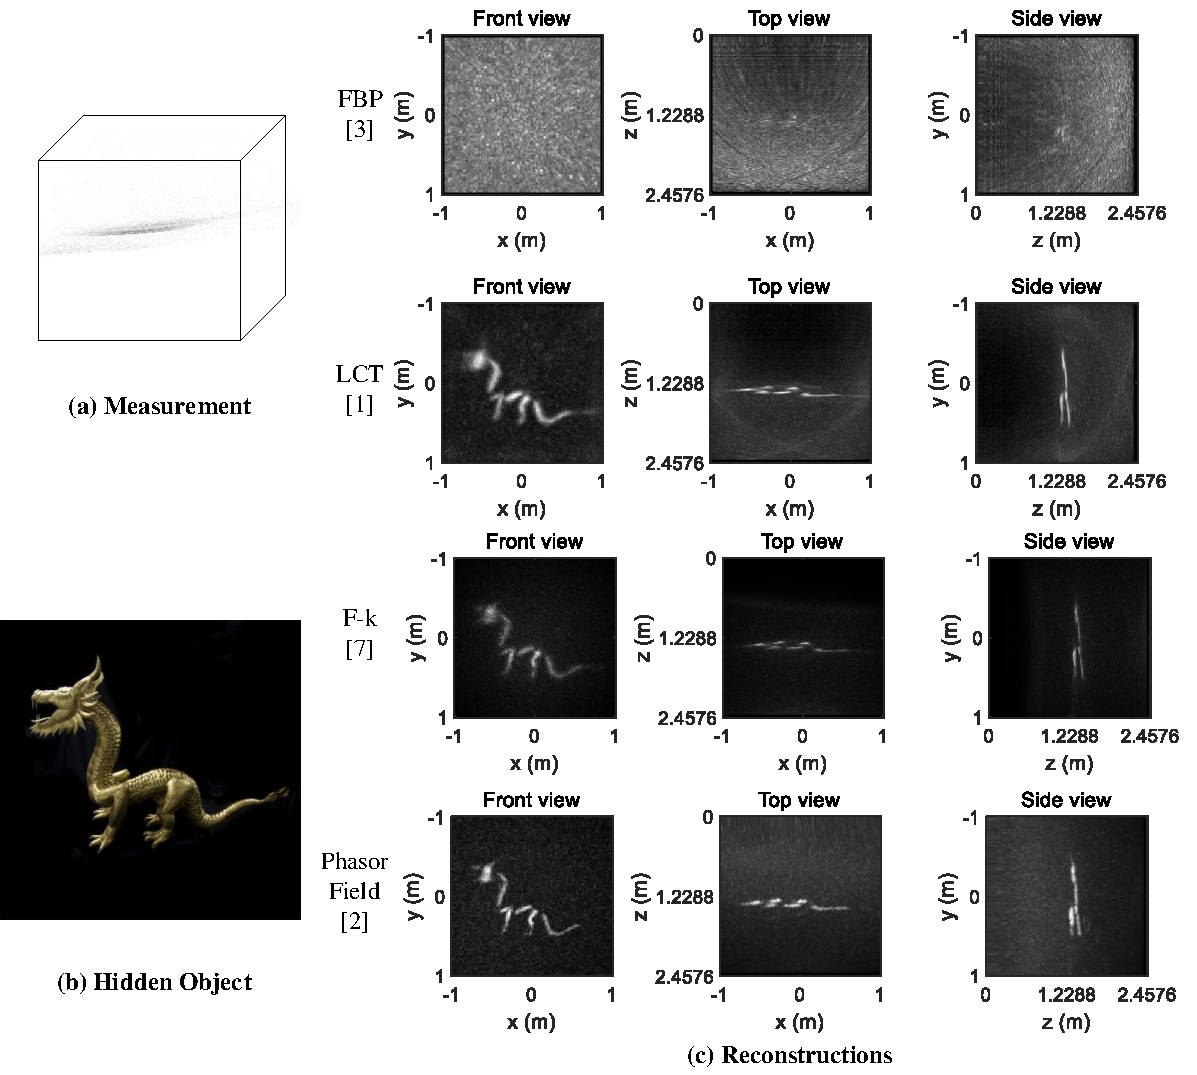
\includegraphics[width=1\textwidth]{./pic/Fig3_activeresult.pdf}%
    \caption{Reconstructions completed by different methods. (a) Measurement data; (b) Hidden object (dragon); (c) Reconstruction results under several typical methods, including FBP~\cite{veltenRecoveringThreedimensionalShape2012}, LCT~\cite{otooleConfocalNonlineofsightImaging2018}, f-k migration~\cite{Lindell:2019:Wave} and phasor field~\cite{liuVirtualWaveOptics2018}. This figure is finished based on the public code and data of \cite{otooleConfocalNonlineofsightImaging2018,o2017reconstructing,heideNonlineofsightImagingPartial2017,Lindell:2019:Wave}.}
    \label{fig:activeresult}
\end{figure*}

\bookmark[dest=\HyperLocalCurrentHref,level=3]{High-level representation}
\subsubsection{High-level representation}
Besides volumetric and surface-based methods, with the rapid development of deep learning in recent years, some works have exploited high-level representation to complete NLOS reconstruction~\cite{chopiteDeepNonLineofSightReconstruction2020,chen_learned_2020}. Specifically, in a data-driven manner, an encoder is used to extract high-dimensional features of the measurement data, while a decoder is used to map them to the hidden object space to complete the reconstruction. Due to the lack of suitable data sets and the incomplete exploration of the network structure, such methods usually have limited generalization capabilities and reconstruction effects. However, compared to traditional reconstruction methods~\cite{otooleConfocalNonlineofsightImaging2018,liuPhasorFieldDiffraction2020,xinTheoryFermatPaths2019,Young:2020:dlct}, the high-level representation methods based on deep learning have faster inference speed (less than 100ms) and stronger feature extraction capabilities, which is a kind of promising methods.

To emphasize the application prospect of deep learning in NLOS imaging, this paper puts all deep learning methods into Sec.~\ref{sec4}. Therefore, please refer to Sec.~\ref{sec4} for detailed discussion and challenges of the high-level representation methods.

\bookmark[dest=\HyperLocalCurrentHref,level=2]{Reconstruction methodology}
\subsection{Reconstruction methodology}
\label{sec:active_reconstruct}
Active reconstruction algorithms can be divided into two categories according to reconstruction methodology: inverse methods and wave-based (forward) methods.

\bookmark[dest=\HyperLocalCurrentHref,level=3]{Inverse methods}
\subsubsection{Inverse methods}
It can be seen from the forward propagation model (Eq.~\ref{eq1}) that what the active NLOS imaging completed is the inverse process, that is to recover the hidden scene $\rho$ from the measurement $\tau(\mu,\mu',t)$. Under the assumptions of isotropic reflection, no interreflection and only three-bounce light, Eq.~\ref{eq1} degenerates into a linear model, which can be solved by a variety of inverse methods (e.g., back projection~\cite{arellanoFastBackprojectionNonline2017,mannaErrorBackprojectionAlgorithms2018,veltenRecoveringThreedimensionalShape2012} and matrix inverse~\cite{heideDiffuseMirrors3D2014,otooleConfocalNonlineofsightImaging2018}).

\vspace{0.8mm}
\noindent \textbf{Back projection}
For general NLOS imaging scenes, the Dirac function in Eq~(\ref{eq2}) essentially represents an ellipsoidal constraint
\begin{equation}
    r + r_l = c t
\end{equation}

The reconstruction of this model is similar to the ellipsoidal Radon transform used in CT. In confocal NLOS imaging, the ellipsoidal constraint degenerates into a spherical constraint, and the corresponding reconstruction also becomes the spherical Radon transform in CT. Therefore, the back projection algorithm can be directly used to complete the NLOS reconstruction task. In 2012, Velten \etal~used the back projection algorithm to complete the NLOS imaging experiment for the first time\cite{veltenRecoveringThreedimensionalShape2012}. Arellano~\etal~reformulated back projection as the voxelization of ellipsoidal space--time manifolds induced by individual three-bounce measurements~\cite{arellanoFastBackprojectionNonline2017}. Rather than evaluating every candidate voxel against every captured sample, the algorithm projects only signal-bearing ellipsoids into the reconstruction volume using the GPU rasterization pipeline. This ellipsoidal-manifold voxelization lowers the dominant computation from voxel-wise accumulation toward measurement-driven processing, scales far more gently with output resolution, and reports speedups of up to three orders of magnitude with negligible reconstruction error. Subsequent iterative error-backprojection methods further refined the residual between simulated and measured transients~\cite{mannaErrorBackprojectionAlgorithms2018}. Since it has been widely used in CT, the back projection algorithm is simple, easy to understand, and has a low space complexity ($O(N^3)$), which can effectively reconstruct simple hidden scenes. However, the back projection algorithm's time complexity is relatively high ($O(N^5)$), and it is difficult to use other prior information, unable to reconstruct a complex optical transport process.

\vspace{0.8mm}
\noindent \textbf{Matrix Inverse.}
In addition to the back projection algorithm based on the ellipsoidal constraint, NLOS reconstruction can also be completed by directly solving the inverse process of Eq.~(\ref{eq2}), that is
\begin{equation}
    \rho = A^{-1}\{\tau\}
    \label{inverse}
\end{equation}
One straightforward approach is to directly solve the pseudo-inverse of the optical transport matrix $A$, such as using the singular value decomposition. Taking singular value decomposition as an example, since the optical transport matrix $A$ is with the size of $N^3 \times N^3$,  the time and space complexity of the algorithm to find the matrix inversion directly is $O(N^{3\times 3=9})$ and $O(N^6)$ respectively, as discussed in \cite{otooleConfocalNonlineofsightImaging2018}.
Another obvious disadvantage of direct inversion is that it is difficult to use the inherent non-negativity, sparsity, and other priors (see Sec. IV-\ref{sec:PriorsinNLOS} for details) in NLOS imaging, leading to bad results. A common alternative is to solve the following optimization problem\cite{heideDiffuseMirrors3D2014} iteratively
\begin{equation}
\rho_{opt}=\underset{\mathbf{\rho}}{\operatorname{argmin}} \frac{1}{2}\|\mathbf{A} \rho -\tau\|_{2}^{2}+\Gamma(\mathbf{\rho})
\label{eqK}
\end{equation}
Among them, $\Gamma(\mathbf{\rho})$ enables this type of iterative inverse method to utilize multiple constraints. Although iterative methods\cite{guptaReconstructionHidden3D2012,buttafavaNonlineofsightImagingUsing2015} can further reduce errors and achieve good reconstruction results, they require multiple iterations, which is still difficult to apply in real-time. O'Toole \etal~\cite{otooleConfocalNonlineofsightImaging2018}~found that under confocal conditions, the forward imaging process can be expressed in the form of three-dimensional convolution, thus using efficient deconvolution algorithms (such as Wiener filtering) to perform the efficient reconstruction. It reduced the time complexity to $O(N^3log(N))$, which greatly improved the reconstruction speed. 

\vspace{0.8mm}
\noindent \textbf{Circular confocal acquisition and transient sinograms.}
Isogawa~\etal~asked whether confocal NLOS could reduce the relay-wall scan itself rather than only accelerate inversion~\cite{isogawaTransientSinograms2020}. Their C$^2$NLOS acquisition samples a one-dimensional circle instead of a dense two-dimensional raster. After the light-cone-transform time reparameterization, each hidden scatterer traces a sinusoid whose amplitude, phase, and offset encode its three-dimensional location; Hough voting, inverse-Radon reconstruction, or compact linear inversion then recover hidden positions and images. This direct extension of confocal LCT and $f$--$k$ migration established structured scan-path design as a route toward rapid NLOS capture, anticipating later sparse, irregular, and learning-based sampling methods.
% 

\vspace{0.8mm}
\noindent \textbf{Super-field-of-view reconstruction by translated PSFs.}
A finite relay scan conventionally restricts reconstruction to the normal space associated with that detection region. Li~\etal~observed that translating the transient point-spread function equivalently shifts the virtual reconstruction region, and introduced spatial-domain encoding to suppress the circular-convolution artifacts that would otherwise corrupt this extension~\cite{liSuperFoVNLOS2026}. Numerical experiments recover multiple targets over nine times the physical detection area, while measured data reconstruct targets beyond twice the single-axis detection range and support stitched coverage equivalent to approximately $19.6\times$ the original area. This work treats field of view as a computational degree of freedom, complementing sparse scanning and non-planar relay methods without requiring a second acquisition aperture.

\vspace{0.8mm}
\noindent \textbf{Adaptive spiral relay-wall sampling.}
Fixed circular and spiral trajectories reduce acquisition relative to dense raster scanning, but they spend the same sampling budget regardless of where a localized hidden target returns useful photons. Oyama~\etal~proposed Dynamic Archimedean Spiral Confocal NLOS, which updates the spiral center from sequential estimates of relay-wall return intensity and concentrates later measurements on informative regions~\cite{oyamaAdaptiveSpiralNLOS2026}. Voronoi density compensation corrects the nonuniform sampling induced by this adaptive path before transient-sinogram reconstruction. The method directly continues C$^2$NLOS from predefined structured paths toward closed-loop measurement allocation.


\vspace{0.8mm}
\noindent \textbf{Model-decomposition reconstruction from sparse transients.}
Sparse transient acquisition reduces scan time but usually shifts the computational burden to large regularized inverse problems. Yang~\etal~formulated MD-NLOS as a spectrally filtered non-negative LASSO problem and decomposed it into smaller updates suited to parallel GPU execution~\cite{yangModelDecompositionNLOS2026}. Their experiments reconstruct $128\times128$ hidden images from only 64 relay measurements in 4.6~s. In the development from analytic LCT and structured scan paths toward learned completion, this work occupies a complementary optimization route: it preserves an explicit linear transport model and sparsity prior while restructuring the solver for practical low-sample latency.

\vspace{0.8mm}
\noindent \textbf{Sparse Bayesian transient restoration.}
Analytic inverses cannot recover temporal detail that has already been buried by photon noise or broadened by the instrument response. Tian~\etal~introduced sparse Bayesian learning as a geometry-independent deconvolution stage before LCT or $f$--$k$ migration~\cite{tianSparseBayesianNLOS2026}. Adaptive sparsity inference suppresses background fluctuations while retaining physically plausible multipath peaks, improving boundary sharpness and robustness without changing the acquisition geometry or downstream reconstruction. This signal-domain route complements spatial undersampling methods by treating transient fidelity itself as a deployment bottleneck.

\vspace{0.8mm}
\noindent \textbf{Frequency-domain regularization experts.}
A single spectral prior is rarely optimal across low-frequency shape, high-frequency boundaries, and scene-dependent noise. Zhang~\etal~formulate active NLOS reconstruction as a frequency-domain mixture of regularization experts and derive expert weights from optimization dual variables rather than heuristic or learned gating~\cite{zhangFrequencyMoENLOS2026}. The resulting solver retains direct-method computational efficiency while improving real-data albedo fidelity and robustness over analytic, iterative, and representative learned baselines.

\vspace{0.8mm}
\noindent \textbf{Reference-free artifact identification and correction.}
Chen~\etal~address backprojection artifacts without ground-truth images or a perfectly matched forward model~\cite{chenCannyArtifactNLOS2026}. Canny edges and morphological closing separate likely object and artifact regions; Tenengrad sharpness and residual energy define a reference-free genetic-algorithm objective; and an optimized blur kernel corrects the measured transient before backprojection. Tests on confocal and non-confocal simulated and measured data show a complementary robustness route based on measurement correction rather than a stronger scene prior.

\vspace{0.8mm}
\noindent \textbf{Inverse Rendering.}
Back projection~\cite{mannaErrorBackprojectionAlgorithms2018,veltenRecoveringThreedimensionalShape2012} and matrix inverse methods~\cite{heideDiffuseMirrors3D2014,otooleConfocalNonlineofsightImaging2018} are both based on voxel representation in reconstruction topology. The voxel-based representation is easy to solve mathematically, but the accuracy is usually low due to ignoring factors such as BRDF and non-Lambert reflections~\cite{tsaiVolumetricAlbedoSurface2019}. On the other hand, by representing the surface of the hidden object, a more accurate forward imaging model (see~\cite{tsaiVolumetricAlbedoSurface2019}) can be established, based on which the optimization methods can be used to solve it to complete the surface reconstruction. Since the imaging models based on surface parameters (such as BRDF and surface normal) rely on rendering, the corresponding reconstruction methods are also referred as inverse rendering, or analysis-by-synthesis. Compared with voxel-based inverse methods, inverse rendering can reconstruct more details, but often requires higher temporal complexity\cite{Young:2020:dlct,heideNonlineofsightImagingPartial2017}.


\vspace{0.8mm}
\noindent \textbf{Beyond volumetric albedo: direct surface optimization.}
Tsai~\etal~introduced a foundational analysis-by-synthesis framework that optimizes hidden surface geometry and reflectance directly, rather than first recovering an unoriented volumetric albedo field~\cite{tsaiVolumetricAlbedoSurface2019}. Their radiometric rendering formulation efficiently computes derivatives of transient measurements with respect to both NLOS shape and reflectance while retaining the underlying multi-bounce transport physics. Coupled with stochastic optimization and geometry-processing regularization, this surface representation reconstructs substantially finer geometric detail than earlier volumetric inversions. It established the explicit surface-optimization branch that later progressed toward physically based transient renderers, analytical differentiable rendering, neural implicit surfaces, self-calibration, and Gaussian transient representations.

\vspace{0.8mm}
\noindent \textbf{Geometry-constrained joint normal and albedo reconstruction.}
Surface orientation supplies geometric and illumination cues that are discarded by a scalar albedo volume, but jointly estimating albedo and normals substantially enlarges the inverse problem. Liu~\etal~regularized hidden normal-field variation through the shape operator and jointly reconstructed surface normals and albedo from transient measurements~\cite{liuGeometricConstrainedNLOS2025}. The method improves geometric detail and robustness on synthetic and measured data while reporting approximately $30\times$ faster optimization than an earlier surface-reconstruction baseline. Its final IEEE TVCG publication formalizes a trajectory from direct surface optimization toward explicit differential-geometric priors for hidden-scene recovery.

\vspace{0.8mm}
\noindent \textbf{Physically based transient analysis-by-synthesis.}
Iseringhausen and Hullin established an early physically grounded inverse-rendering formulation for transient NLOS surface reconstruction~\cite{iseringhausen:2018}. Instead of backprojecting measurements into an unoriented voxel volume, their method represents the hidden object as an implicit level-set surface, renders wall--object--wall transport with a custom GPU transient renderer, and globally optimizes the scene to match measured transients. The forward model explicitly includes surface orientation, BRDF-dependent scattering, shading, visibility, and self-occlusion, allowing detailed recovery under substantial noise and non-diffuse reflectance. This analysis-by-synthesis milestone supplied the conceptual and computational bridge from surface optimization to later differentiable transient renderers, neural transient fields, self-calibrating inverse rendering, and Gaussian transient scene representations.

\vspace{0.8mm}
\noindent \textbf{Fast differentiable transient rendering.}
Plack~\etal~introduced a physically based differentiable transient renderer tailored to NLOS reconstruction~\cite{plackFastDifferentiableTransient2023}. By making gradients through time-resolved light transport efficient enough for consumer hardware, their analysis-by-synthesis pipeline reduces inverse-rendering runtimes from hours to minutes while improving optimization stability. The same renderer also supports self-supervised learning, forming an important bridge between explicit transient inverse rendering and later self-calibrating or learned NLOS reconstruction pipelines.

\vspace{0.8mm}
\noindent \textbf{Self-calibrating differentiable NLOS inverse rendering.}
Choi~\etal~closed a complementary deployment gap by coupling phasor-field volumetric reconstruction in the frequency domain with differentiable path-space transient rendering in the temporal domain~\cite{choiSelfCalibratingNLOS2023}. Starting only from measured transients, the end-to-end pipeline ray-marches the reconstructed volume to extract hidden surface points and normals, then jointly optimizes virtual-illumination and diffraction-filter parameters, the combined laser--sensor temporal response, and per-surface albedo by minimizing the discrepancy between rendered and measured transients. This self-calibration removes much of the manual filter and hardware-response tuning required by earlier wave-based pipelines, improves geometry and reflectance recovery under substantial noise, and forms a direct methodological bridge from efficient differentiable transient rendering to later neural-field and Gaussian transient representations.

\bookmark[dest=\HyperLocalCurrentHref,level=3]{Wave-based methods}
\subsubsection{Wave-based methods}
\label{sec:waveBased}
The theoretical basis of the three types of algorithms mentioned above is geometric optics. Besides that, wave-based methods have also achieved rapid development in recent years.
Lindell \etal~described NLOS imaging as a wave propagation problem in three-dimensional space. Inspired by inverse methods used in seismology, it completed NLOS imaging using f-k migration\cite{Lindell:2019:Wave}. In that work, referring $\Psi(x,y,z,t)$ as the field in 3D space as a space-time function, the NLOS reconstruction is converted as 
\begin{equation}
    \Psi(x, y, z=0, t) \quad \Rightarrow \quad \Psi(x, y, z, t=0)
\end{equation}
where $\Psi(x, y, z=0, t)$ and $\Psi(x, y, z, t=0)$ can be regarded as the available measurement data and the hidden target scene, respectively. 
With $t=0$, the functions $\Phi$ and $\Psi$ in Eq.~\ref{eqwave_3} are related by a Fourier transform. By replacing $dk_z$ with $d_f$ and using Stolt interpolation, Eq.~\ref{eqwave_3} can be converted to another representation. In the new representation, when z = 0, functions $\Phi$ and $\Psi$ are again a pair connected by Fourier transform. In this way, taking $\Psi(x, y, z=0, t)$ as input, the hidden scene $\Psi(x, y, z , t=0)$ can be easily reconstructed through three steps: 3D Fourier transform, Stolt interpolation, and inverse 3D Fourier transform. Strictly speaking, f-k migration~\cite{Lindell:2019:Wave} is an inverse method (reconstruction through the reverse process of forward propagation). However, compared to other typical inverse methods such as back projection~\cite{arellanoFastBackprojectionNonline2017,veltenRecoveringThreedimensionalShape2012}, matrix inverse~\cite{heideDiffuseMirrors3D2014} and inverse rendering~\cite{tsaiVolumetricAlbedoSurface2019}, f-k migration does not have an obvious inversion process (e.g., ADMM~\cite{otooleConfocalNonlineofsightImaging2018}), but is more like a forward process completed in the frequency domain.


Besides, Liu~ \etal~\cite{liuPhasorFieldDiffraction2020,liuVirtualWaveOptics2018}~and Reza~\etal~\cite{rezaPhasorFieldWaves2019}~introduced virtual wave phasor to NLOS imaging. Based on the phasor field, NLOS imaging can be transformed into a LOS optical imaging problem and then solved by the existing algorithm in diffraction imaging. 
Different from other methods, phasor field methods~\cite{liuPhasorFieldDiffraction2020,liuVirtualWaveOptics2018} transform the relay wall into a virtual aperture (or lens of any LOS system). The reconstruction is the diffraction integral of the wavefront of the virtual aperture, which is equivalent to the forward propagation process of the measurement data. Therefore, phasor field methods~\cite{liuPhasorFieldDiffraction2020,liuVirtualWaveOptics2018} do not need to reverse the forward process like inverse methods~\cite{otooleConfocalNonlineofsightImaging2018,veltenRecoveringThreedimensionalShape2012} -- they can directly complete the reconstruction through wavefront propagation.

\vspace{0.8mm}
\noindent \textbf{Virtual light-transport analysis.}
Marco~\etal~extended phasor-field virtual wave optics beyond hidden-geometry reconstruction by constructing computational projector--camera pairs and estimating a virtual light transport matrix of the hidden scene~\cite{marcoVirtualLightTransport2021}. Probing this matrix enables virtual relighting and separates direct, first-order indirect, and higher-order indirect illumination in cluttered NLOS scenes, showing that transient NLOS measurements can support light-transport analysis as well as geometric imaging.

\vspace{0.8mm}
\noindent \textbf{Visibility limits and recoverability.}
Beyond developing faster inverses, Liu~\etal~analyzed which hidden-scene features are physically visible in transient NLOS measurements~\cite{liuAnalysisFeatureVisibility2019}. Their study connects recoverability to surface orientation, finite relay-wall aperture, and acquisition geometry, explaining why some surfaces remain weak or absent even under accurate reconstruction. This visibility perspective established an important limit-aware complement to LCT, $f$--$k$ migration, and phasor-field propagation, and motivates later methods that explicitly model normals, occlusion, and adaptive capture.

\vspace{0.8mm}
\noindent \textbf{Finite-aperture yaw observability.}
Romanelli~\etal~characterized how a finite sampled relay wall limits orientation recovery in confocal transient NLOS~\cite{romanelliFiniteApertureYawNLOS2026}. A geometric switch-line criterion identifies when the endpoint ordering that supports unique planar reconstruction leaves the measured aperture, while a Fisher-information analysis shows that yaw sensitivity decays continuously rather than disappearing abruptly. Simulated and experimental $f$--$k$ and backprojection results connect this loss of angular information to edge-like or spatially ambiguous reconstructions. The study turns the qualitative missing-cone and feature-visibility limitation into quantitative guidance for relay-wall size, placement, and pose estimation.

\vspace{0.8mm}
\noindent \textbf{Stereo relay-wall acquisition.}
The missing cone is not only an algorithmic artifact: with one finite relay aperture, surfaces whose orientations direct little transport toward that aperture remain intrinsically weak. Luesia-Lahoz~\etal~introduced a stereo NLOS configuration with two distinct relay walls and used phasor fields to treat both as generalized virtual camera apertures~\cite{luesiaStereoNLOS2026}. The reconstruction combines measurements that illuminate and detect on the same wall with cross-wall paths that illuminate one wall and observe the other. These complementary angular views improve conditioning, diminish missing-cone artifacts, and provide surface-orientation cues from the relative wall contributions, extending phasor-field imaging from a single virtual aperture to coordinated multi-aperture capture.

\vspace{0.8mm}
\noindent \textbf{Reference-function phase compensation for non-confocal capture.}
Non-confocal acquisition improves photon use and capture speed but produces bistatic path geometry that is less convenient for confocal Fourier inverses. Yu~\etal~transferred a single-input/multiple-output frequency-domain imaging formulation from millimeter-wave sensing and derived a reference-function phase compensation method for optical NLOS~\cite{yuNonconfocalPhaseCompensation2026}. FFT implementation reduces computation while measured and simulated results show fewer artifacts and less geometric distortion. The work provides an explicit RF-to-optical algorithmic bridge rather than using radar only as an application analogy.

\vspace{0.8mm}
\noindent \textbf{Specular-flight-path regularization.}
Non-confocal measurements provide flexible capture but can become highly redundant for complex tilted objects. Shi~\etal~use local matrix analysis to identify specular-flight-path regions with lower column similarity and information redundancy, then regularize inversion around those paths~\cite{shiSpecularFlightPathNLOS2026}. The method improves simulated and measured reconstruction for multi-orientation hidden scenes, showing that path selection can condition the inverse problem before generic spatial regularization is applied.

The wave-based approaches have two attractive advantages: (1) It is more robust to the material of the relay surface; (2) It can easily combine NLOS imaging with other related fields, such as LOS imaging and seismic imaging. These advantages, as well as the phase acquisition problem in wave-based approaches, are explained in detail in Faccio \etal's review\cite{faccioNonlineofsightImaging2020}.

\vspace{0.8mm}
\noindent \textbf{Extensions to Non-Planar Relay Surfaces.}
The classical ToF and wave-based models assume a planar relay wall, restricting applicability to flat, vertical surfaces. Gu~\etal~proposed a fast algorithm that generalizes confocal NLOS reconstruction to arbitrary non-planar relay surfaces by transforming the measurements to an equivalent planar configuration, enabling efficient FFT-based reconstruction even when the relay geometry deviates from a plane~\cite{guNonPlanar2023}. Similarly, Liu~\etal~introduced a Bayesian framework with confocal-complemented signal-object collaborative regularization (CC-SOCR) that handles arbitrary illumination and detection patterns on the relay surface without requiring a regular grid~\cite{liuNLOSArbitraryIllumination2023}, greatly broadening the applicability of NLOS systems to irregular or partial relay surfaces encountered in real-world scenarios.

Moving from arbitrary relay sampling toward extreme measurement sparsity, Liu~\etal~introduced signal-surface collaborative regularization (SSCR), which jointly regularizes the photon-event signal, a three-dimensional voxel representation, and a two-dimensional hidden-surface representation~\cite{liuFewShotSSCR2022}. The method supports both confocal and non-confocal acquisition and reconstructs complex hidden geometry from as few as $5\times5$ confocal measurements, showing how mixed-dimensional physical priors can replace much of the dense raster scan required by earlier transient NLOS systems.

\vspace{0.8mm}
\noindent \textbf{Higher-Order Bounce Imaging.}
Standard transient NLOS reconstruction usually truncates transport at the third bounce, which limits visibility for unfavorably oriented surfaces and confines most systems to a single corner. Royo~\etal~showed that planar diffuse surfaces behave specularly at the computational wavelengths of the phasor-field domain and can therefore act as ``virtual mirrors''~\cite{royoVirtualMirrors2023}. By propagating measured transients to these surfaces and constructing secondary virtual apertures, their method recovers limited-visibility geometry and objects hidden behind a second corner without requiring physical specular reflectors. This result shifts higher-order light transport from a discarded nuisance to an additional imaging resource.

\vspace{0.8mm}
\noindent \textbf{Phasor Fields under Scattering Conditions.}
The phasor field framework assumes a clean relay surface, but in practice the relay surface may be contaminated by scattering media (e.g., dust, fog). Luesia~\etal~systematically analyzed the behavior of phasor-field NLOS reconstruction under such scattering conditions, identifying the mechanisms that degrade performance and proposing modifications to improve robustness~\cite{luesiaPhaso2022}. This study provides important design guidelines for practical NLOS systems operating in non-ideal environments.

It should be noted that not all of the above algorithms are suitable for confocal settings. Specifically, FBP~\cite{arellanoFastBackprojectionNonline2017,veltenRecoveringThreedimensionalShape2012}, phasor field~\cite{liuPhasorFieldDiffraction2020,liuVirtualWaveOptics2018}, and matrix inverse methods~\cite{heideDiffuseMirrors3D2014} are applicable to all NLOS systems. In contrast, LCT~\cite{otooleConfocalNonlineofsightImaging2018} and f-k migration~\cite{Lindell:2019:Wave} are only applicable to confocal NLOS systems. \cite{Lindell:2019:Wave} proposed a conversion method from non-confocal data to confocal data, so that confocal algorithms can also be used to reconstruct non-confocal data. From the perspective of time complexity, for confocal settings, a series of algorithms after LCT~\cite{otooleConfocalNonlineofsightImaging2018} (including f-k migration~\cite{Lindell:2019:Wave}) can reach the time of $O(N^3logN)$ complexity due to the efficient calculation of FFT in the frequency domain, while only the phasor field algorithm~\cite{liuPhasorFieldDiffraction2020} can achieve the same temporal complexity for non-confocal NLOS scenes.
Figure~\ref{fig:activeresult} illustrates the measurement with a dragon as the hidden scene, and the reconstruction results obtained by different reconstruction methods~\cite{otooleConfocalNonlineofsightImaging2018,veltenRecoveringThreedimensionalShape2012,liuVirtualWaveOptics2018,Lindell:2019:Wave}. It can be seen that existing methods can already reconstruct complex hidden scenes. In general, the wave-based methods~\cite{liuVirtualWaveOptics2018,Lindell:2019:Wave} are more suitable for hidden scenes with rich details.


\bookmark[dest=\HyperLocalCurrentHref,level=3]{Transformer and Neural Representation-Based Methods}
\subsubsection{Transformer and Neural Representation-Based Methods}
\label{sec:transformerNeural}
Motivated by the success of transformers and implicit neural representations in computer vision, recent works have brought these advances into NLOS reconstruction.

\vspace{0.8mm}
\noindent \textbf{Transformer-based reconstruction.}
Li~\etal~proposed NLOST, the first transformer-based network for NLOS reconstruction~\cite{liNLOST2023}. NLOST extracts shallow features with physics-based priors, then employs two spatial-temporal self-attention encoders to capture both local and global correlations within 3D NLOS measurement volumes at different scales. A cross-attention decoder integrates these features, enabling superior reconstruction of complex hidden scenes on both confocal and non-confocal real-world data. Building on this line, Yu~\etal~proposed enhancing physics-based NLOS reconstruction by introducing a learnable inverse kernel in the Fourier domain combined with an attention mechanism, allowing the network to better capture high-frequency details that are difficult to recover due to spectral bias~\cite{yuEnhancingLearnable2023}. On the sensor side, Cho~\etal~proposed to enhance the aperture phasor field representation using a learned network, achieving state-of-the-art performance~\cite{choAperturePhasor2024}, while Shim~\etal~introduced a domain reduction strategy that identifies the most likely occupied regions in the 3D volume and focuses reconstruction effort there, reducing computational cost by an order of magnitude~\cite{shimDomainReduction2024}.

\vspace{0.8mm}
\noindent \textbf{Neural implicit surface reconstruction.}
Fujimura~\etal~proposed NLOS-NeuS, extending neural transient fields to neural implicit surfaces with a signed distance function (SDF) representation~\cite{fujimuraNLOSNeuS2023}. By incorporating SDF constraints derived from first-returning photon geometry, NLOS-NeuS enables smooth yet detailed 3D surface reconstruction in NLOS scenes, overcoming the voxel resolution limitation of volumetric methods. This represents the first neural implicit surface approach with volume rendering for NLOS scenes.

\vspace{0.8mm}
\noindent \textbf{Joint LOS/NLOS holistic shape reconstruction.}
Huang~\etal~introduced Omni-LOS, which combines direct LOS transients and diffuse-wall NLOS transients in a unified neural level-set representation~\cite{huangOmniLOS2023}. The method derives differentiable rendering models for straight LOS rays and spherical NLOS wavefronts, jointly optimizing visible front surfaces and self-occluded back geometry from a fixed scan position. With nearby walls acting as diffuse virtual mirrors and a SPAD--laser prototype, Omni-LOS recovers near-$360^\circ$ object shape without a surrounding camera or mirror rig, extending neural transient imaging from hidden-scene reconstruction toward holistic single-position 3D scanning.

\vspace{0.8mm}
\noindent \textbf{Diffusion model-based reconstruction.}
Su~\etal~proposed a model-guided iterative diffusion sampling framework for NLOS reconstruction~\cite{suModelGuidedDiffusion2024}. Starting from the back-projection result, the diffusion model iteratively refines the reconstruction while respecting the NLOS physical forward model as a consistency constraint. This approach achieves physically consistent reconstructions with high visual quality, benefiting from the strong generative prior of diffusion models while avoiding hallucination artifacts.

\bookmark[dest=\HyperLocalCurrentHref,level=3]{Detection, location and identification}
\subsubsection{Detection, location and identification}
Under some scenarios, we do not necessarily need to complete the difficult but low-level task of imaging/ reconstruction. On the contrary, some  high-level vision tasks, such as detection, localization, and recognition of hidden objects, are needed. For the detection task, we only need to judge whether there is a peak in the measurement data. 
For localization tasks, a naive but effective algorithm is back projection\cite{chanNonlineofsightTrackingPeople2017a,gariepyDetectionTrackingMoving2016}. Through back projection, the distribution probability of objects in three-dimensional space can be established to determine the object's position. Compared with the reconstruction task, the localization task can greatly reduce the number of scanning points and the resolution of discrete voxels with much less reconstruction time and space complexity. 

For recognition tasks, traditional algorithms are limited by their ability to understand high-level semantics, making it difficult to map from experimental data to label results directly.
Therefore, NLOS recognition is typically  based on data-driven methods (see Sec.~\ref{sec4} for details).

\vspace{0.8mm}
\noindent \textbf{Real-measurement hidden-human detection.}
Celebi and Turkoglu built an active SPAD--TCSPC NLOS sensing system and collected transient waveforms for hidden people across multiple poses, orientations, and rubble-like object configurations~\cite{celebiHumanDetectionNLOS2026}. CNN, GRU, and random-forest models all detected the human-present class with full sensitivity, while the random forest achieved the strongest specificity and weighted F1 under the available photon statistics. This result complements image reconstruction and tracking by showing that low-cost transient hardware can support a high-level search-and-rescue decision directly from measured histograms, without first recovering a detailed hidden scene.


\begin{figure*}[!h]
    \centering
    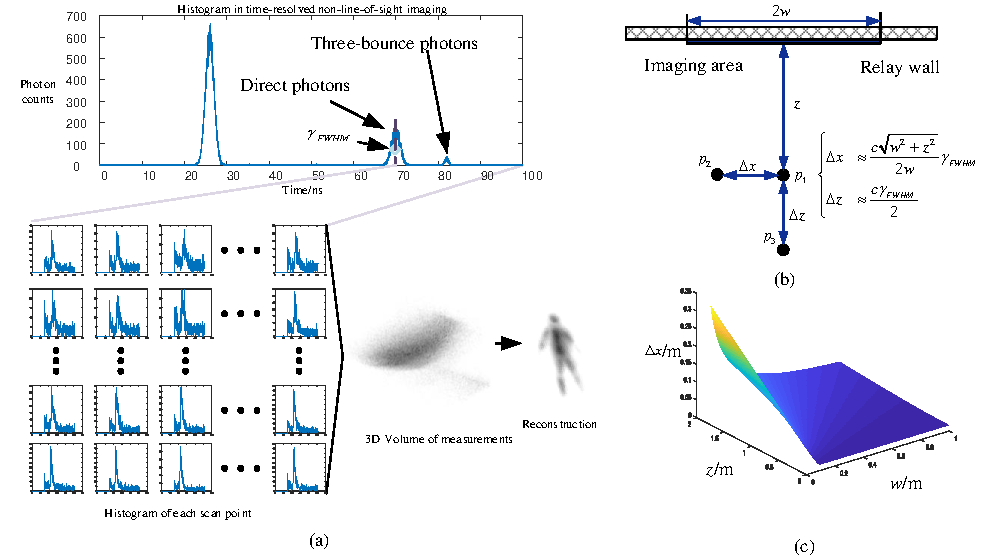
\includegraphics[width=1\textwidth]{./pic/Fig4_resolution.pdf}%
    \caption{The principle and spatial resolution of active (confocal) NLOS imaging. (a) The detector receives the photon arrival time histogram at each point, and these histograms form a 3D Volume of measurements $\tau$, which can be used to recover the hidden object (albedo) $\rho$. The measurement data is from \cite{otooleConfocalNonlineofsightImaging2018}. (b) The resolution of the imaging system. (c) The influence of the distance between the object and the wall $z$ and the scan area size $w$ on the horizontal resolution $\Delta x$.}
    \label{fig:active}
\end{figure*}


\bookmark[dest=\HyperLocalCurrentHref,level=2]{Challenges and Prospects}
\vspace{0.8mm}
\noindent \textbf{Irregular, aperture-limited, and under-scanned relay measurements.}
Recent work increasingly relaxes the dense planar-wall assumption. DO-NLOS~\cite{miaoUnderScanning2025} combines convolution approximation and optimization for strongly under-scanned measurements; sub-pixel resolving modulation~\cite{zhangSubpixelModulation2025} extracts spatial detail beyond the native relay sampling grid; and CUDA-accelerated reconstruction on irregular relay surfaces~\cite{sunCUDAIrregular2026} makes geometry-aware filtered backprojection practical on modern GPUs. These developments complement self-supervised Virtual Scanning and diffusion-based transient completion by improving the physical solver and acquisition model rather than relying only on learned interpolation.

\subsection{Challenges and Prospects} \label{sec:activeChallenge}
Despite considerable progress in recent years, active NLOS imaging still faces many challenges, including ill-posedness with low SNR, limited resolution, and long data acquisition time. 

\bookmark[dest=\HyperLocalCurrentHref,level=3]{Ill-posedness with low SNR}
\subsubsection{Ill-posedness with low SNR}
Since the collected effective signal is three-bounce of reflected light, and the signal intensity has an attenuation of $r^2\sim r^4$\cite{otooleConfocalNonlineofsightImaging2018} (varies with different reflective materials) with distance $r$, the signal strength is weak. In many NLOS scenes (such as long-distance imaging\cite{wuNonLineofsightImaging2021,liSinglephotonImaging2002021}), the echo can reach the order of a single photon. On the other hand, there are various kinds of noise. All of the dark count and after-pulse of SPAD, the pile-up effect of TCSPC, and the ambient light can cause noise. Therefore, NLOS imaging tasks have a very low SNR, which makes NLOS imaging very challenging. Moreover, hidden objects in different locations may contribute the same measurement value\cite{liuAnalysisFeatureVisibility2019}, which further exacerbates the problem's ill-posedness.

The methods of improving the SNR have been discussed in \cite{liSinglephotonImaging2002021,wuNonLineofsightImaging2021,Li:20}, including improving the receiving device to increase the detection efficiency and thus the signal strength, combining  spatial filtering with multimode fiber, spectral filtering with narrow-band filters and temporal filtering through gate-mode SPAD, and using polarizers to minimize noise. Based on the above methods, an amazing 1.43km NLOS imaging can be achieved. In addition to improving the signal-to-noise ratio from the hardware, it is also important to improve the reconstruction algorithm to alleviate the ill-posedness through various prior constraints, such as the sparsity, non-negativity, surface normal, partial occlusion (as discussed in Sec.~\ref{activeAlg}) and the recently developed data-driven scene prior (see in Sec.~\ref{sec4}).


\bookmark[dest=\HyperLocalCurrentHref,level=3]{Long data acquisition time}
\subsubsection{Long data acquisition time}
\label{sec:longDataAcqui}
Active NLOS imaging requires a full raster scan of a relay wall. This point-by-point scanning mechanism leads to long data acquisition time, which hinders real-time NLOS imaging applications. Current work usually uses a multifunction I/O device (e.g., NI DAG USB-6343) to control the galvanometer mirrors (e.g., Thorlabs GVS012) to scan point by point and completes the event synchronization with the photon counter(e.g., TCSPC, PicoHarp 300). Limited by the scanning speed of the galvanometer and the minimum number of photons at each point, the scanning frequency is only 1Hz to 10Hz (depending on the imaging conditions) in state-of-the-art NLOS systems, such as LCT\cite{otooleConfocalNonlineofsightImaging2018} and f-k migration~\cite{Lindell:2019:Wave}. When the number of scanning points is $64\times 64$, the scanning speed of less than 10Hz is difficult to complete real-time data acquisition.

\begin{figure*}[!h]
    \centering
    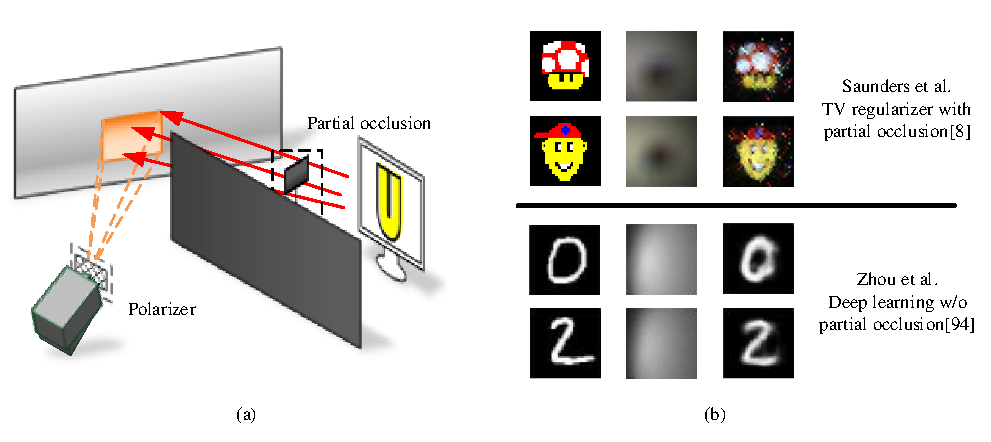
\includegraphics[width=1\textwidth]{./pic/Fig5_passive.pdf}%
    \caption{Passive NLOS imaging: (a) Common constraints in passive NLOS imaging; (b) Passive NLOS imaging results.}
    \label{fig:passive}
 \end{figure*}

\vspace{0.8mm}
\noindent \textbf{Reducing scanning points.}
In theory, each scan point in NLOS imaging contains the whole hidden object's shape information. Therefore, although reducing the scan points would inevitably reduce the imaging quality, it is possible only to scan a few points to complete the imaging task. Liu \etal~studied the impact of randomly removing some test points on the reconstruction results~\cite{liuRoleWignerDistribution2020}. Ye \etal~applied compressed sensing to NLOS imaging, and only $5\times 5$ points can achieve a resolution of $64\times 64$,  thereby greatly reducing the time required for scanning~\cite{yeCompressedSensingActive2021}. Isogawa \etal~further changed the scanning methods, using the circular scanning path, and proposed $C^2NLOS$(Circular and confocal NLOS)~\cite{isogawaEfficientNonLineofSightImaging}. $C^2NLOS$ improved the limit of the scanning speed of the galvanometer through circular scanning and reduced the number of scanning points, thereby reducing the data acquisition time.

More recently, CVPR 2023 established two complementary routes to extreme sparse acquisition: SSCR uses mixed-dimensional optimization priors, while Wang~\etal~proposed a signal superresolution network that maps sparse scanning measurements to dense ones before reconstruction, achieving a $16\times$ reduction in acquisition time while maintaining comparable quality~\cite{liuFewShotSSCR2022,wangSignalSuperresolution2023}. Li~\etal~then proposed the first deep learning framework specifically for NLOS reconstruction from under-scanning measurements (USM), using a transient recovery network (TRN) to recover full-density transients from sparse inputs, followed by a physical-model-based volume reconstruction network (VRN) that achieves $50\times$ faster reconstruction than iterative methods~\cite{liDeepUnderscanning2023}. Cui~\etal~introduced Virtual Scanning, an unsupervised framework for NLOS reconstruction from irregularly undersampled transients without requiring paired ground truth, leveraging a physics-guided denoiser to handle the noise inherent in low-photon conditions~\cite{cuiVirtualScanning2024}.

From the detection side, Li~\etal~proposed FPES (First Photon Event Stamping), which records only the first detected photon at each scan point~\cite{liFastFirstPhoton2022}. By exploiting the Poisson statistics of single-photon arrival, FPES achieves comparable reconstruction quality with up to $10\times$ fewer total photons, enabling faster acquisition in photon-starved scenarios. Similarly, Liu~\etal~developed a photon-efficient NLOS approach that achieves robust reconstruction with fewer than one photon per pixel on average~\cite{liuPhotonEfficientNLOS2022}.

\vspace{0.8mm}
\noindent \textbf{SPAD array.}
In addition to reducing the scanning points, the development of SPAD array to achieve scannerless NLOS imaging is a very promising direction. There have been the latest researches that develop algorithms suitable for SPAD array~\cite{liuPhasorFieldDiffraction2020,nam_real-time_2020} or directly use  $32\times 32$ SPAD camera to complete scannerless NLOS imaging~\cite{jinScannerlessNonlineofsightThree2020}.
Multiple lasers simultaneously illuminating would cause crosstalk problems, which is unacceptable. Therefore, the current NLOS imaging systems based on SPAD array all adopt the structure of "one laser, multiple pixels". In essence, this is equivalent to multiple parallel conventional non-confocal NLOS imaging systems. Therefore, any algorithm suitable for non-confocal reconstruction, including but not limited to back projection~\cite{arellanoFastBackprojectionNonline2017}, f-k migration~\cite{Lindell:2019:Wave} and phasor field, can be used in NLOS imaging systems based on SPAD array.~\cite{jinScannerlessNonlineofsightThree2020} verified that the reconstruction quality using commercial SPAD array based on phasor field~\cite{liuPhasorFieldDiffraction2020} is close to the early single-pixel NLOS imaging~\cite{veltenRecoveringThreedimensionalShape2012}.

Zhang~\etal~demonstrated a real-time scan-free NLOS imaging system achieving up to 19\,fps by combining single-pixel detection with structured illumination (SPAD array) and computational reconstruction, and further demonstrated robustness to outdoor daylight conditions~\cite{zhangRealTimeScanFree2024}. Towards real-time NLOS video of room-sized dynamic scenes, Ye~\etal~proposed a framework of spectrum filtering and motion compensation, achieving 4\,fps NLOS video reconstruction of real-life dynamic scenes through denoising in the frequency domain and interleaved scanning~\cite{yeRealTimeNLOS2024}. This landmark result marks a major step towards practical deployment. Further, Li~\etal~developed TransiT, a transient transformer architecture for NLOS videography that reconstructs $64\times64$ resolution videos at 10\,fps from $16\times16$ sparse transient measurements via transfer learning to bridge the synthetic-to-real domain gap~\cite{liTransiT2025}.

Before these later dynamic systems, Nam~\etal~combined two gated $16\times1$ SPAD arrays (28 active pixels), sparse relay-wall scanning, virtual-aperture remapping, and fast Rayleigh--Sommerfeld phasor-field propagation to acquire and reconstruct diffuse, non-retroreflective hidden scenes at $5\,\mathrm{fps}$ with approximately $1\,\mathrm{s}$ latency~\cite{nam_real-time_2020}, providing an early full-pipeline real-time NLOS video milestone.

\vspace{0.8mm}
\noindent \textbf{Steady-state imaging.}
Another possible alternative is to replace the pulsed laser with a steady-state laser~\cite{chenSteadystateNonLineofSightImaging2019} or even an ordinary condensing light source (such as a projector)~\cite{chandranAdaptiveLightingDataDriven2019} and use a conventional camera to collect the imaging area directly. These steady-state methods usually rely on data-driven deep learning methods for reconstruction, which will be discussed in Sec.~\ref{sec4}. Zhu~\etal~proposed a two-step deep remapping framework that first remaps sparse non-confocal transients to dense confocal equivalents, then applies standard reconstruction algorithms, achieving a 4$\times$ speedup over FK migration while maintaining quality~\cite{zhuTwoStepRemapping2022}. Mu~\etal~combined a physics-based forward model with deep learning to enable high-speed NLOS reconstruction from significantly fewer and noisier measurements, demonstrating reconstruction at up to 5\,fps, a $10\times$ improvement over prior approaches~\cite{muphysicsrescue2022}. Snapshot NLOS acquisition---capturing hidden scene information from a single camera frame without scanning---has also advanced. Seidel~\etal~demonstrated a snapshot corner camera that reconstructs both hidden foreground objects and background scenes without laser scanning from a single optical response model~\cite{seidelSnapshot2023}.

\bookmark[dest=\HyperLocalCurrentHref, level=3]{Limited resolution}
\subsubsection{Limited resolution}
Like LiDAR and Radar, the resolution of NLOS imaging is also divided into axial resolution $\Delta z$ and transverse resolution $\Delta x$. Time jitter $\gamma$, the time domain response of the imaging system greatly influences $\Delta x$, and it also determines $\Delta z$. $\gamma$ mainly depends on the detector's temporal resolution, laser pulse width, laser spatial divergence, and other components. In the recent long-distance NLOS imaging research~\cite{wuNonLineofsightImaging2021}, the time jitter $\gamma$ has been formulated. Another factor of $\Delta x$ is the size of the scanning area (
equivalent to the size of the aperture). Usually, we use $w$ to represent the radius of the scanning area, as shown in Fig.~\ref{fig:active}-(b). For a confocal system, the resolution of the system in two directions $\Delta z$ and $\Delta x$ are~\cite{otooleConfocalNonlineofsightImaging2018}

\begin{equation}
    \begin{cases}
    \Delta x& \approx \frac{c \sqrt{w^{2}+z^{2}}}{2 w} \gamma_{FWHM}\\
    \Delta z& \approx \frac{c \gamma_{FWHM}}{2}
    \end{cases}
    \label{res}
\end{equation}

Among them, $\gamma_{FWHM}$ refers to the full width at half maximum (FWHM) of the time jitter $\gamma$, as illustrated in Fig.~\ref{fig:active}-(a). From Fig.~\ref{fig:active}-(c), it can be seen that reducing the time jitter $\gamma$ and increasing the size of the scanning area $w$ are effective ways to improve the confocal system resolution.
For other active NLOS scenes, \cite{kadambiOccludedImagingTimeofflight2016,liuAnalysisFeatureVisibility2019,buttafavaNonlineofsightImagingUsing2015} discussed the limits of spatial resolution. \cite{liuAnalysisFeatureVisibility2019} also analyzed how the position and the normal direction of the hidden object affect the imaging results from the Fourier domain.

Beyond improving temporal resolution, recent works have tackled the challenge of long-range NLOS imaging. The groundbreaking active-focusing approach UNCOVER~\cite{caohighresolutionnlos2022} achieves $\sim0.6\,\text{mm}$ resolution at 0.55\,m, demonstrating that diffraction-limited NLOS imaging is attainable via wavefront shaping. At the system level, coherent sensing with frequency-comb calibration~\cite{huangCoherentNLOS2024} enables NLOS imaging under strong ambient illumination conditions where incoherent ToF methods fail, additionally demonstrating the novel capability of NLOS vibrometry---remotely measuring vibrations of hidden objects. These advances substantially broaden the conditions under which active NLOS systems can operate in real-world outdoor environments.
